% gold-price-2024.tex
% English recreation of the 2024 gold price trend report (2 pages, A4).
% Layout and figures match the Chinese source; numbers are unchanged.
\documentclass[11pt,a4paper]{article}

\usepackage[a4paper,top=1.6cm,bottom=1.8cm,left=1.6cm,right=1.6cm]{geometry}
\usepackage[T1]{fontenc}
\usepackage[utf8]{inputenc}
\usepackage{lmodern}
\usepackage{fancyhdr}
\usepackage{booktabs}
\usepackage{colortbl}
\usepackage{xcolor}
\usepackage{array}
\usepackage{tabularx}
\usepackage{graphicx}
\usepackage{pgfplots}
\usepackage{caption}
\usepackage{setspace}
\usepackage{parskip}
\usepackage{tikz}

\pgfplotsset{compat=1.18}
\usetikzlibrary{calc}

% Palette close to the source (pale gold / beige)
\definecolor{headerbg}{RGB}{250,243,214}
\definecolor{tableborder}{RGB}{201,179,106}
\definecolor{sectiongold}{RGB}{176,141,60}
\definecolor{linegold}{RGB}{212,168,58}
\definecolor{chartbg}{RGB}{252,247,230}
\definecolor{muted}{RGB}{110,110,110}
\definecolor{bodytext}{RGB}{40,40,40}

\pagestyle{fancy}
\fancyhf{}
\renewcommand{\headrulewidth}{0.4pt}
\renewcommand{\footrulewidth}{0.3pt}
\fancyhead[L]{\footnotesize\color{muted}Gold Price Review\,|\,Data for study purposes only}
\fancyhead[R]{\footnotesize\color{muted}Page~\thepage~of~2}
\fancyfoot[C]{}
\setlength{\headheight}{14pt}

\captionsetup{font={footnotesize,color=muted},labelformat=empty,skip=4pt}
\setlength{\parskip}{0.45em}
\setlength{\parindent}{0pt}
\color{bodytext}

% Section headings in gold, matching the source style
\newcommand{\secgold}[1]{%
  \vspace{0.55em}%
  {\large\color{sectiongold}\textbf{#1}}\par
  \vspace{0.15em}%
}

\begin{document}

% ---------- Title ----------
\begin{center}
  {\LARGE\bfseries 2024 Gold Price Trend Report}\\[0.45em]
  {\small\color{muted}USD per troy ounce, month-end close basis}
\end{center}
\vspace{0.35em}

% ---------- Summary table ----------
\renewcommand{\arraystretch}{1.35}
\begin{center}
\begin{tabular}{|>{\centering\arraybackslash}p{0.17\textwidth}
               |>{\centering\arraybackslash}p{0.17\textwidth}
               |>{\centering\arraybackslash}p{0.18\textwidth}
               |>{\centering\arraybackslash}p{0.18\textwidth}
               |>{\centering\arraybackslash}p{0.15\textwidth}|}
\hline
\rowcolor{headerbg}
{\footnotesize Year-start} &
{\footnotesize Year-end} &
{\footnotesize Range high} &
{\footnotesize Range low} &
{\footnotesize YTD change} \\
\hline
{\small \$2,039.15} &
{\small \$2,624.60} &
{\small Oct \$2,746.70} &
{\small Jan \$2,039.15} &
{\small +28.7\%} \\
\hline
\end{tabular}
\end{center}

\vspace{0.4em}

% ---------- Chart ----------
\begin{center}
{\small 2024 International Gold Month-End Close}\\[0.2em]
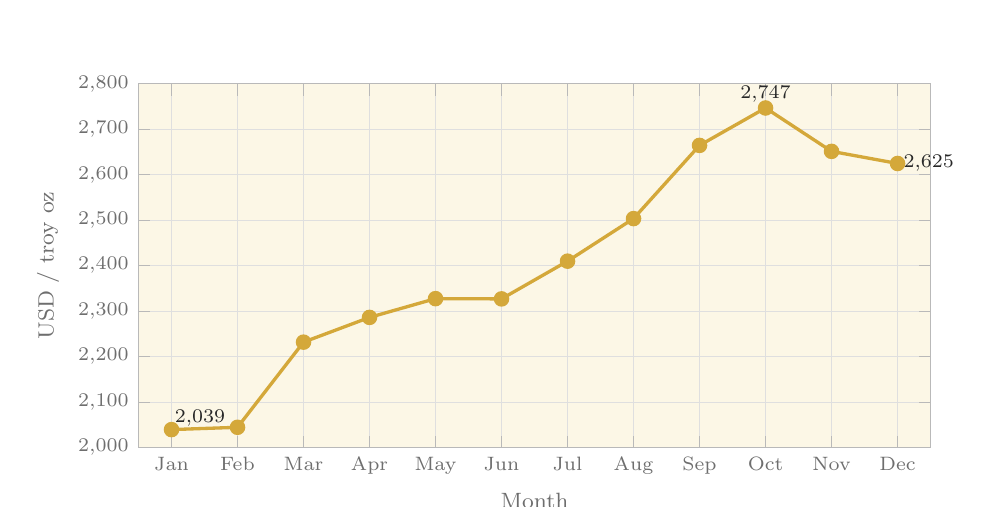
\begin{tikzpicture}
\begin{axis}[
  width=0.96\textwidth,
  height=6.2cm,
  ymin=2000, ymax=2800,
  xmin=0.5, xmax=12.5,
  xtick={1,2,3,4,5,6,7,8,9,10,11,12},
  xticklabels={Jan,Feb,Mar,Apr,May,Jun,Jul,Aug,Sep,Oct,Nov,Dec},
  ytick={2000,2100,2200,2300,2400,2500,2600,2700,2800},
  ylabel={USD / troy oz},
  xlabel={Month},
  ylabel style={font=\footnotesize,color=muted},
  xlabel style={font=\footnotesize,color=muted},
  tick label style={font=\scriptsize,color=muted},
  axis background/.style={fill=chartbg},
  grid=major,
  grid style={gray!25, very thin},
  axis line style={gray!55},
  tick style={gray!55},
  enlargelimits=false,
  clip=false,
]
\addplot[
  color=linegold,
  very thick,
  mark=*,
  mark size=2.2pt,
  mark options={fill=linegold, draw=linegold},
] coordinates {
  (1,2039.15)
  (2,2044.20)
  (3,2231.56)
  (4,2285.99)
  (5,2327.28)
  (6,2326.72)
  (7,2409.69)
  (8,2503.38)
  (9,2664.41)
  (10,2746.70)
  (11,2651.25)
  (12,2624.60)
};
% Labels only at Jan / Oct / Dec (rounded as in the source figure)
\node[anchor=south west, font=\scriptsize, color=bodytext, inner sep=1pt]
  at (axis cs:1,2039.15) {2,039};
\node[anchor=south, font=\scriptsize, color=bodytext, inner sep=2pt]
  at (axis cs:10,2746.70) {2,747};
\node[anchor=west, font=\scriptsize, color=bodytext, inner sep=2pt]
  at (axis cs:12,2624.60) {2,625};
\end{axis}
\end{tikzpicture}
\end{center}
{\footnotesize\color{muted}Figure: Month-end closing prices. For readability, only year-start, year-end, high, and low months are labeled.}

\secgold{I.\ Annual Overview}

2024 was a textbook trending bull market: prices broke above \$2,200 in Q1, kept climbing through Q2 and Q3, then settled near \$2,746.70 at end-October before pulling back from the highs.

Month-end closes rose from about \$2,039.15 in January to about \$2,624.60 in December---a gain of roughly 28.7\% for the year.

Drivers clustered around continued central-bank buying, rate-cut pricing, geopolitical uncertainty, concerns over the dollar's credit and fiscal backdrop, and improved gold ETF/investment demand.

According to the World Gold Council: the 2024 LBMA PM gold price set 40 fresh highs over the year, the annual average was about \$2,386.2/oz, up roughly 23\% year over year, and the Q4 average was about \$2,663/oz.

\secgold{II.\ Phase-by-Phase Changes}

\renewcommand{\arraystretch}{1.25}
\begin{center}
\begin{tabular}{|>{\centering\arraybackslash}p{0.12\textwidth}
               |>{\raggedright\arraybackslash}p{0.78\textwidth}|}
\hline
\rowcolor{headerbg}
{\footnotesize\textbf{Phase}} &
{\footnotesize\textbf{Moves and main drivers}} \\
\hline
{\footnotesize Jan--Feb} &
{\footnotesize Gold range-bound above \$2,000 as markets waited for a clearer Fed rate-cut path.} \\
\hline
{\footnotesize Mar--May} &
{\footnotesize Breakout underway; March month-end already near \$2,231.56, May near \$2,327.28.} \\
\hline
{\footnotesize Jun--Sep} &
{\footnotesize Consolidation at elevated levels, then another push higher; September month-end reached about \$2,664.41.} \\
\hline
{\footnotesize Oct--Dec} &
{\footnotesize October month-end near \$2,746.70 marked the phase high; prices eased slightly in November--December but stayed elevated.} \\
\hline
\end{tabular}
\end{center}

\clearpage

% ---------- Page 2 ----------
\secgold{III.\ Monthly Data Table}

\renewcommand{\arraystretch}{1.35}
{\fontsize{6.5pt}{8pt}\selectfont
\begin{center}
\setlength{\tabcolsep}{1.6pt}
\begin{tabular*}{\textwidth}{|@{\extracolsep{\fill}}c|*{12}{c}|}
\hline
\rowcolor{headerbg}
\textbf{Month} &
\textbf{Jan} & \textbf{Feb} & \textbf{Mar} & \textbf{Apr} &
\textbf{May} & \textbf{Jun} & \textbf{Jul} & \textbf{Aug} &
\textbf{Sep} & \textbf{Oct} & \textbf{Nov} & \textbf{Dec} \\
\hline
Month-end close &
\$2,039.15 & \$2,044.20 & \$2,231.56 & \$2,285.99 &
\$2,327.28 & \$2,326.72 & \$2,409.69 & \$2,503.38 &
\$2,664.41 & \$2,746.70 & \$2,651.25 & \$2,624.60 \\
\hline
\end{tabular*}
\end{center}
}

\secgold{IV.\ Basis Notes and Sources}

{\small
\begin{itemize}
  \setlength{\itemsep}{0.25em}
  \setlength{\parsep}{0pt}
  \item Monthly chart: month-end closes from Macrotrends Gold Prices -- 100 Year Historical Chart.
  \item Annual averages / demand backdrop: World Gold Council \emph{Gold Demand Trends: Full Year 2023/2024} and publicly available LBMA information.
  \item Unit: USD per troy ounce. This is a retrospective review, not investment advice.
\end{itemize}

\vspace{0.4em}
{\color{muted}Generated: 2026-06-07. Range amplitude: \$707.55. Annual average (reference): \$2,386.20.}
}

\end{document}
